%!TEX encoding = UTF-8 Unicode
% -*- coding: UTF-8; -*-
% vim: set fenc-utf-8

\chapter{Diagrammes d'état}
\label{s:diagrammes_etats}

\section{Diagramme d'état d'un joueur}
\label{sec:diagramme_etat_joueur}

\begin{figure}[htpb]
    \centering
    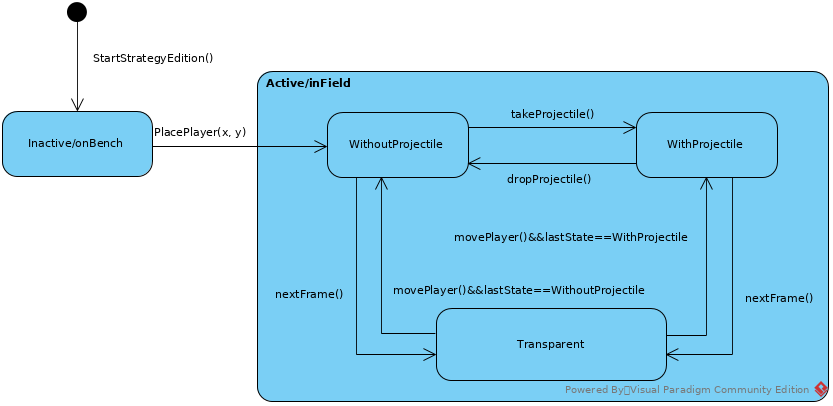
\includegraphics[scale=0.32]{fig/state_diag_player.png}
    \caption{Diagramme d'état d'un joueur}
    \label{fig:state_diag_player}
\end{figure}

La figure \ref{fig:state_diag_player} représente le diagramme d'état d'un joueur lors de l'édition de la stratégie.
Au démmarage de la simulation, les joueurs sont inactifs.
Cela est équivalent à l'idée que les joueurs sont << sur le banc >>.
Placer les joueurs sur le terrain les mets en mode actif.
Lorsqu'un des joueurs a l'état << hasProjectile >>, le projectile change d'état, tel que démontré dans la figure \ref{fig:state_diag_projectile}.
Aussi, le nombre maximum de joueur pouvant avoir cet état  en même temps est limité par le nombre de projectiles sur le terrain.
En mode d'édition image par image, créer un nouvelle image mets tous les joueurs sur le terrain en mode transparent.
Le joueur revient à son état précédent si l'utilisateur fait une action sur le joueur.

\section{Diagramme d'état d'un projectile}
\label{sec:diagramme_etat_projectile}

\begin{figure}[htpb]
    \centering
    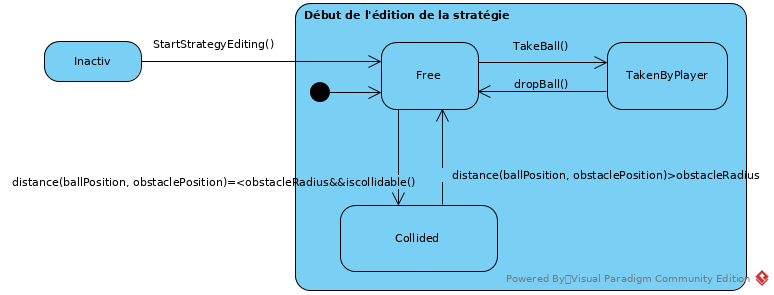
\includegraphics[scale=0.32]{fig/state_diag_projectile.png}
    \caption{Diagramme d'état d'un projectile}
    \label{fig:state_diag_projectile}
\end{figure}

La figure \ref{fig:state_diag_projectile} représente le diagramme d'état d'un projectile lors de l'édition d'une stratégie.
Le projectile sera inactif si l'application n'est pas en mode édition, que ce soit image par image ou temps réel.
L'état de la gestion de la collision doit respecter deux conditions.
Il faut que le projectile << colle >> un obstacle, soit que la distance entre l'obstacle et le projectile est plus petit que le rayon de l'obstacle.
De plus, il faut que l'obstacle ait l'option << gère les collisions >>.
Sinon, le projectile se déplace comme si l'obstacle n'existait pas.

